\documentclass{beamer}
\usepackage[utf8]{inputenc}
\usepackage[T1]{fontenc}
\usepackage{listings}

\graphicspath{{img/}{problem/}{build/}{./}}

\title[Autonomous Calibration]{\large {Autonomous Calibration}\\ of 3D Computer Vision System}
\date{WASP Positioning Sales Pitch}
% \author[Gustaf]{Gustaf Waldemarson \texttt{gustaf.waldemarson@arm.com}}

\usetheme{ulund}

\lstloadlanguages{[ISO]C++}
\lstdefinestyle{google-c++}{%
  language = {[ISO]C++},
  captionpos = {t},
  frame = {lines},
  columns = {fixed},
  numbers = {left},
  numberstyle = {\tiny},
  numbersep = {5pt},
  breaklines = {true},
  basicstyle = {\footnotesize},
  identifierstyle = {\ttfamily},
  keywordstyle = {\color[rgb]{0, 0, 1}},
  commentstyle = {\color[rgb]{0.026,0.112,0.095}},
  stringstyle = {\color[rgb]{0.627,0.126,0.941}},
  numberstyle = {\color[rgb]{0.205, 0.142, 0.73}},
  backgroundcolor = {\color[rgb]{0.9, 0.9, 0.9}},
}


\begin{document}

\begin{frame}
  \titlepage
\end{frame}


\begin{frame}{Cameras for Autonomous Systems}
  \begin{columns}
    \begin{column}{0.5\columnwidth}
      \begin{figure}
        \centering
        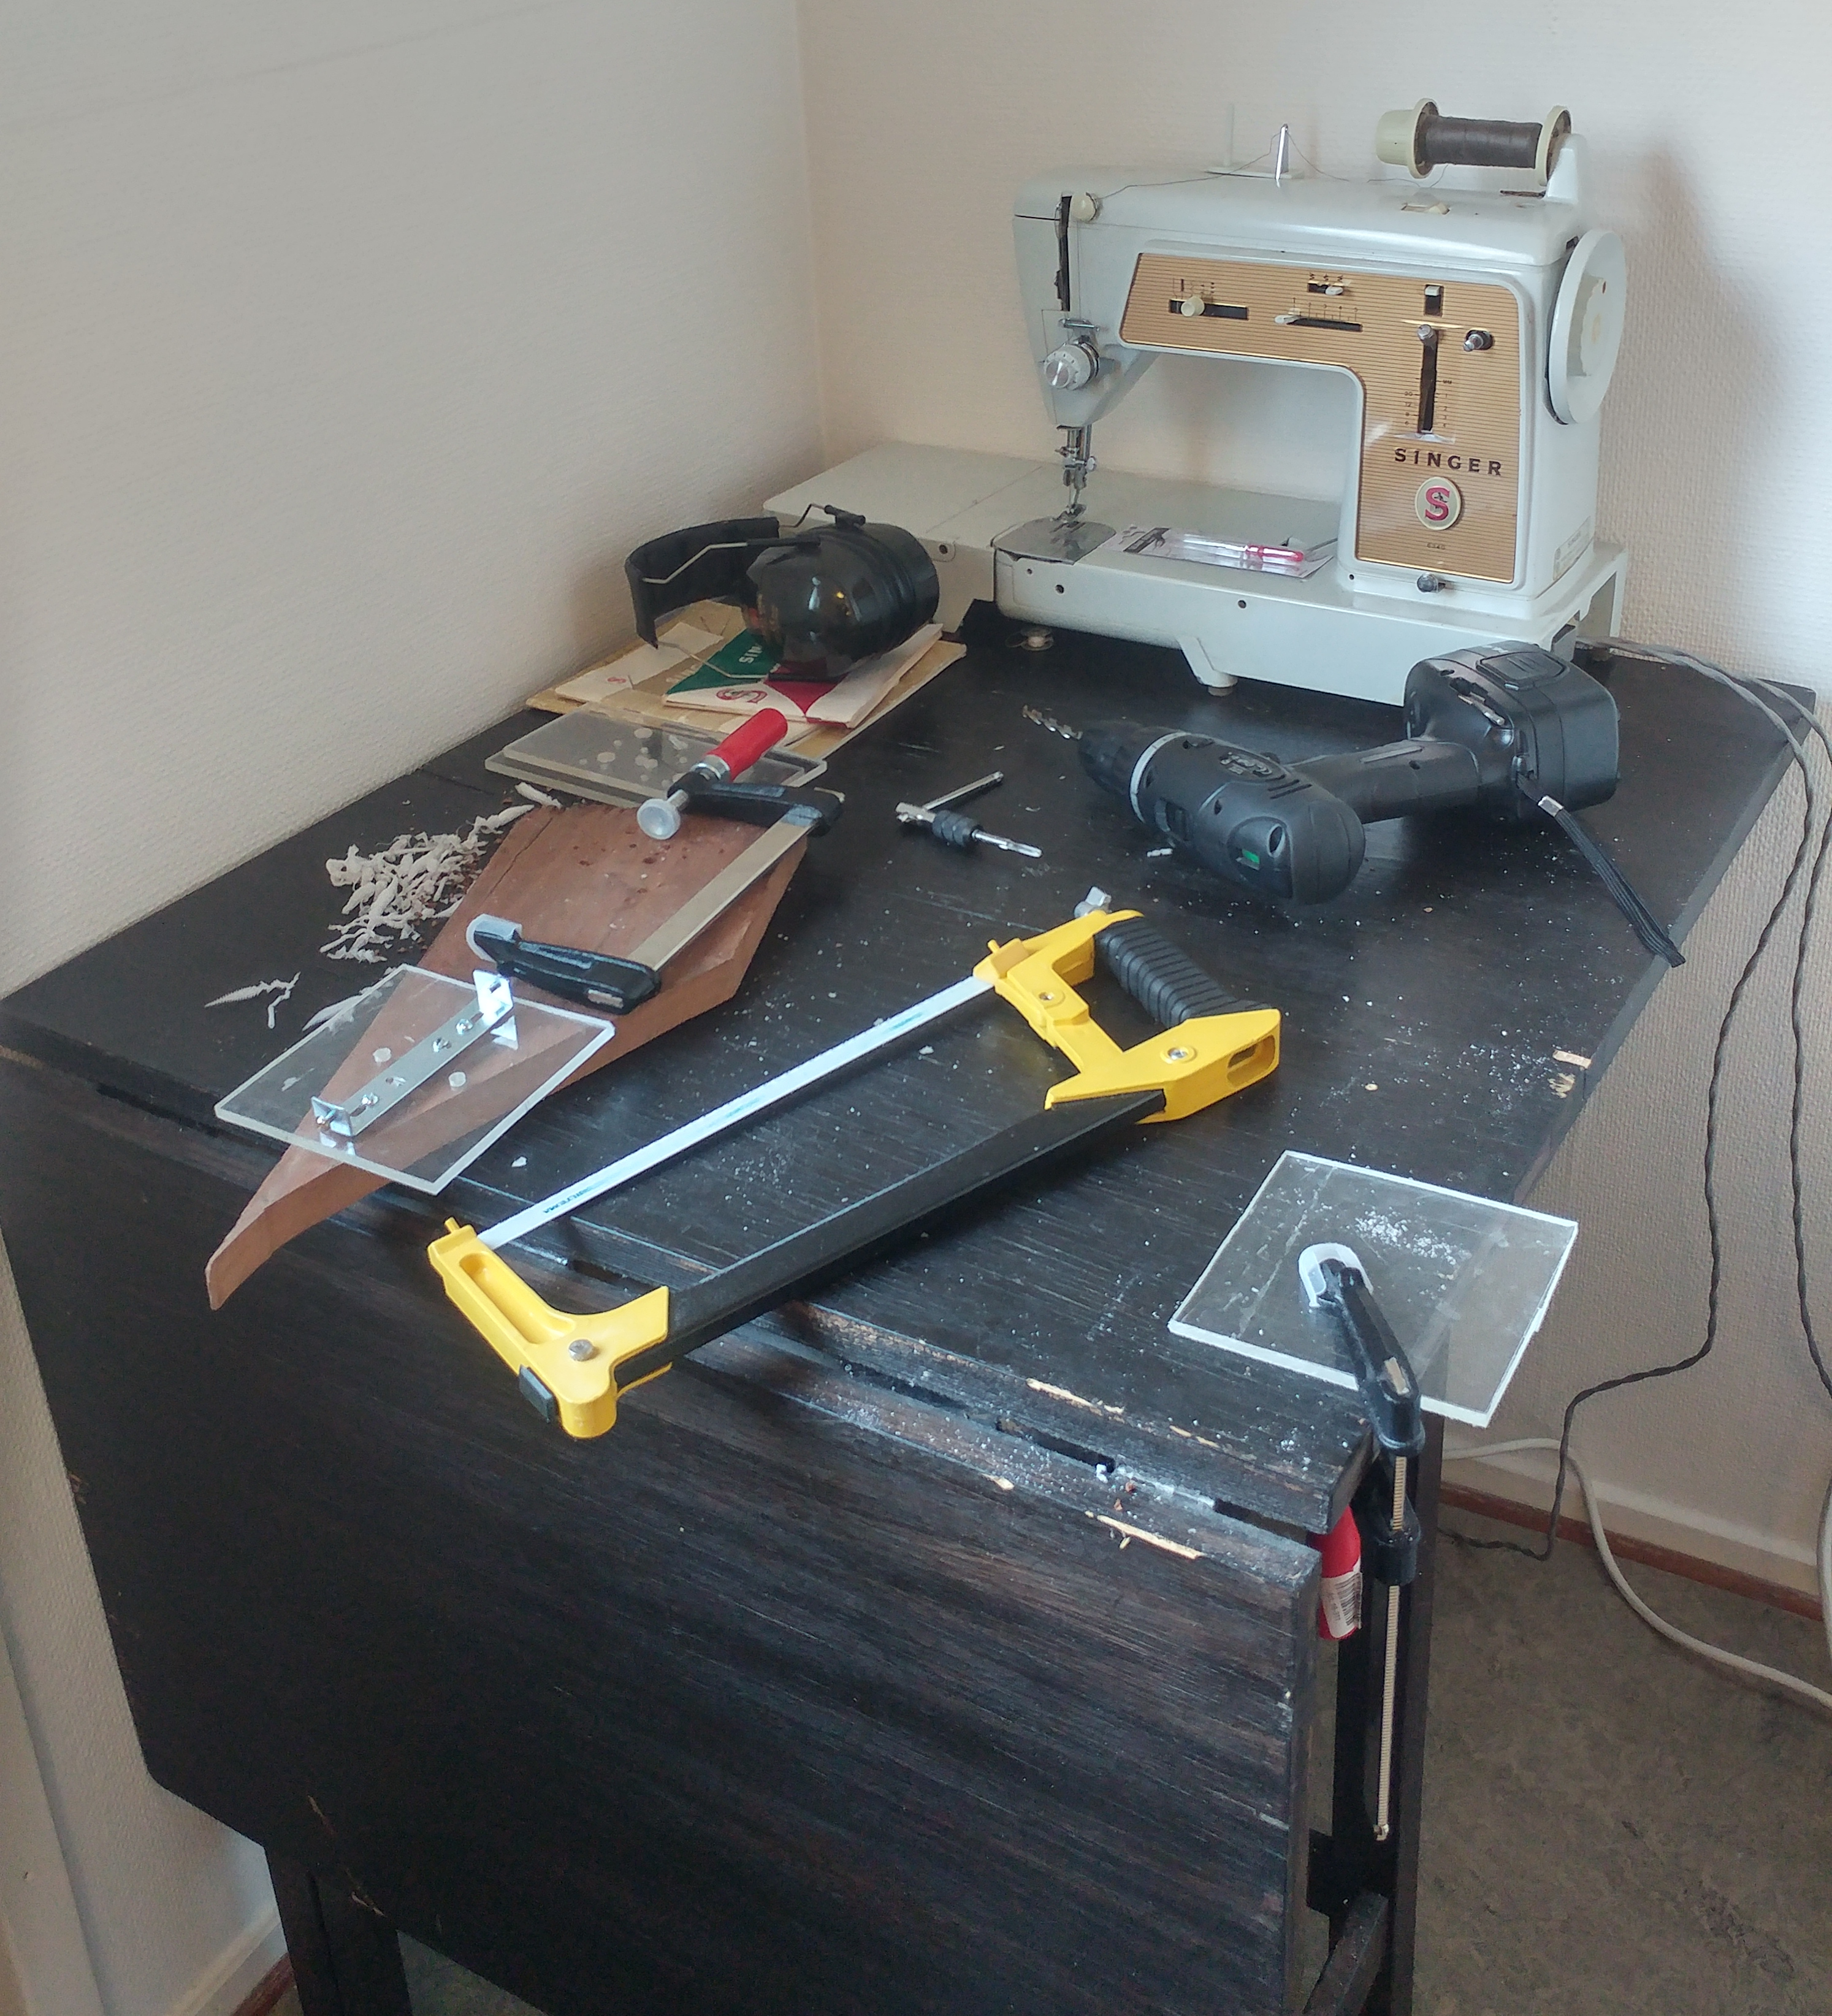
\includegraphics[width=1.0\textwidth]{problem/recog}
      \end{figure}
    \end{column}
    \begin{column}{0.5\columnwidth}
      \begin{figure}
        \centering
        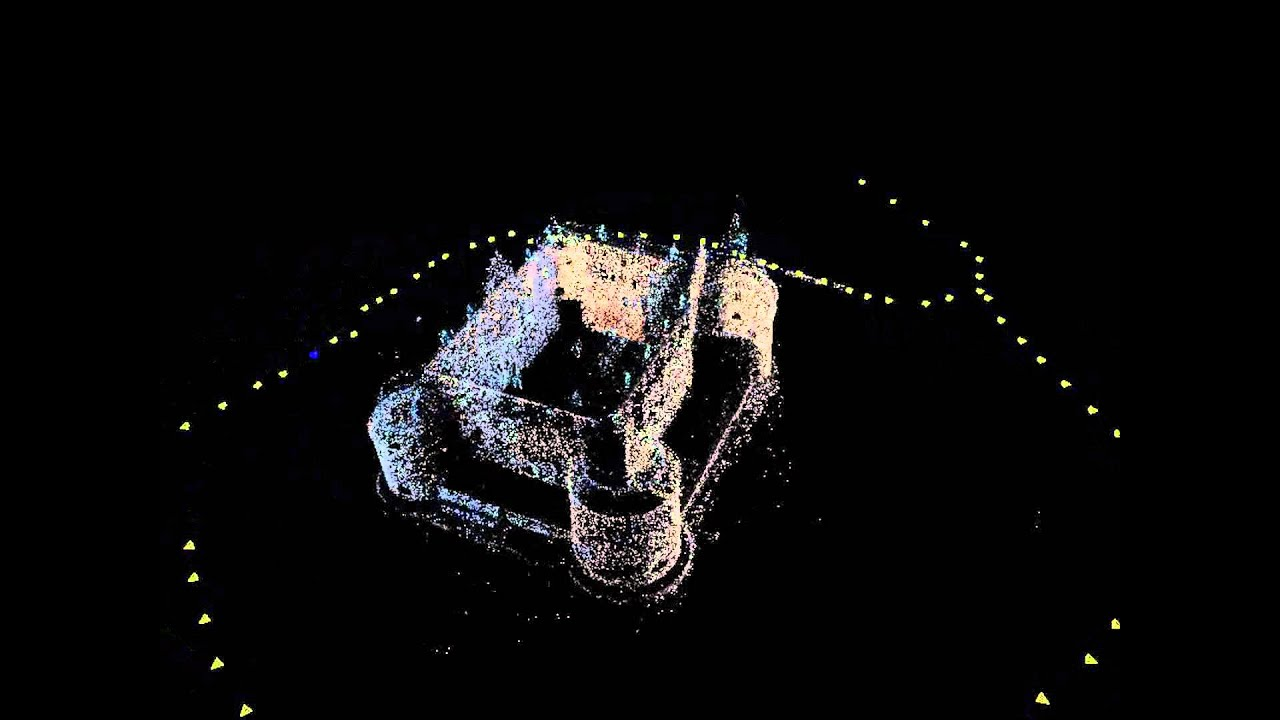
\includegraphics[width=1.0\textwidth]{problem/sfm}
      \end{figure}
    \end{column}
  \end{columns}
\end{frame}


\begin{frame}{The Pin-Hole Camera Model}
  \begin{figure}
    \centering
    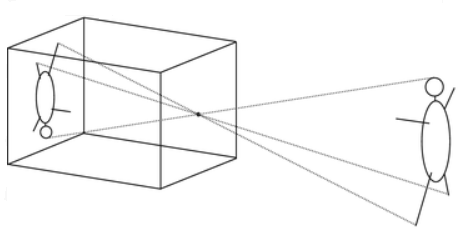
\includegraphics[width=1.0\textwidth]{problem/pinhole}
  \end{figure}
\end{frame}


\begin{frame}{Calibration with Checkerboard Patterns}
  \begin{figure}
    \centering
    
\includegraphics[width=0.7\textwidth]{problem/checkerboard_radon}
  \end{figure}
\end{frame}


\begin{frame}{Cameras for Autonomous Systems}
  \begin{columns}
    \begin{column}{0.5\columnwidth}
      \begin{figure}
        \centering
        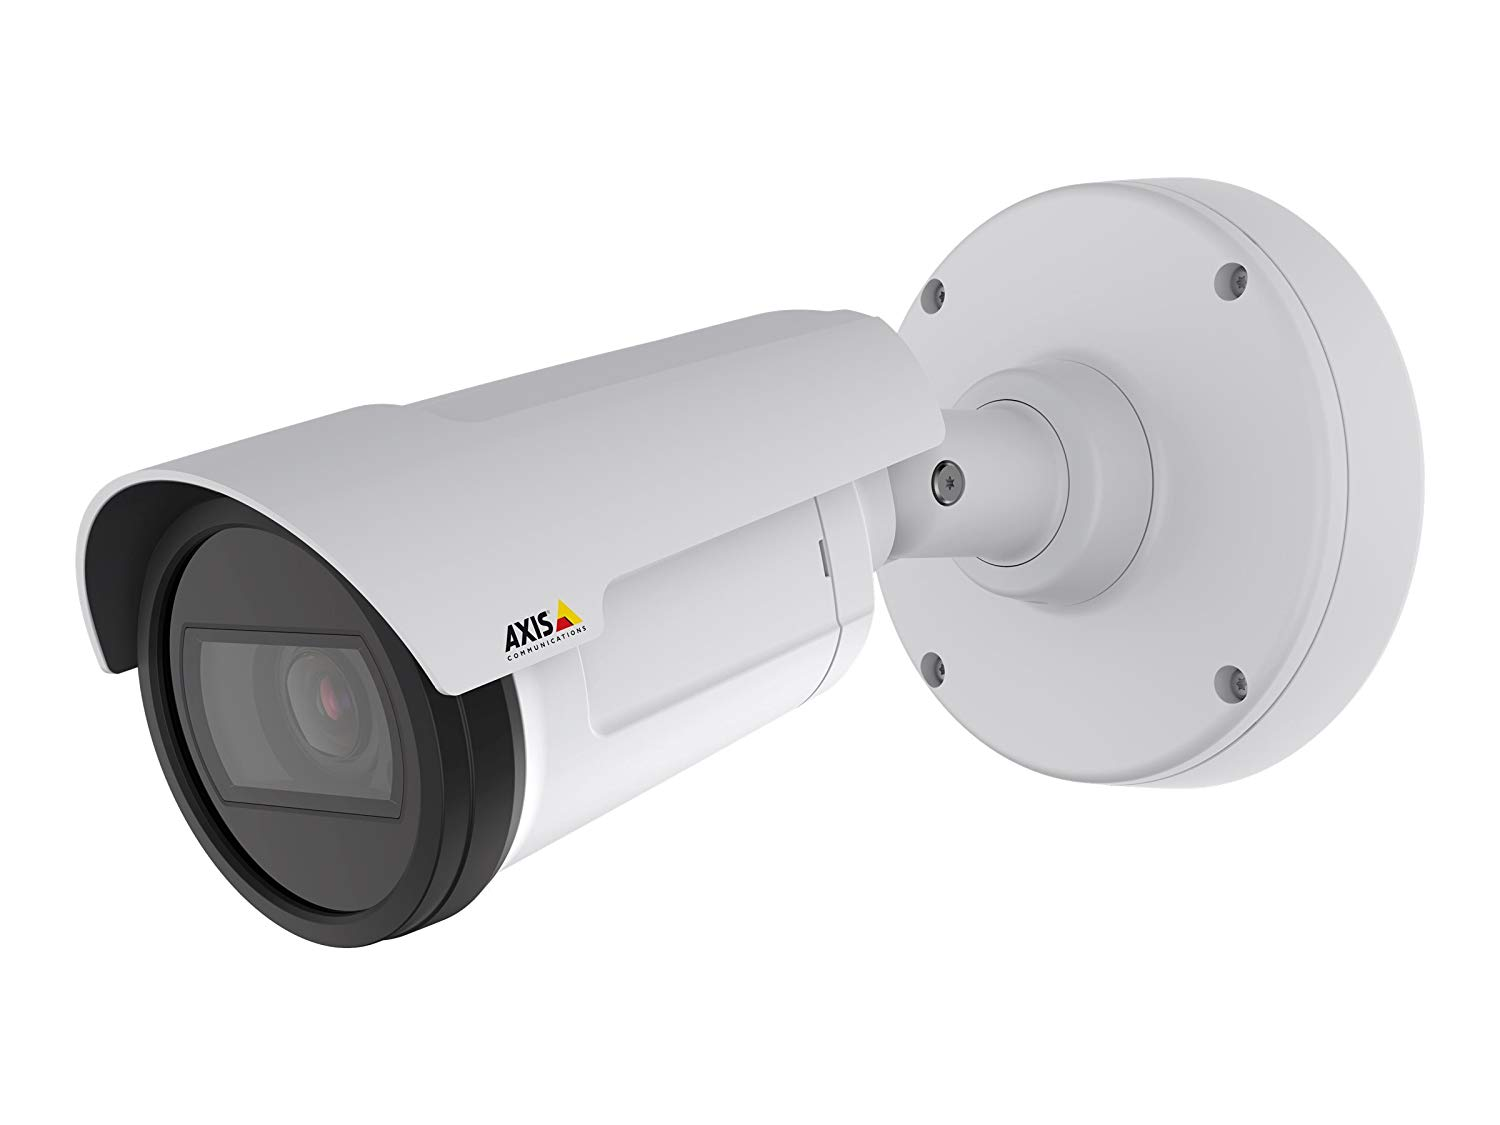
\includegraphics[width=1.0\textwidth]{problem/axis_cam}
      \end{figure}
    \end{column}
    \begin{column}{0.5\columnwidth}
      \begin{figure}
        \centering
        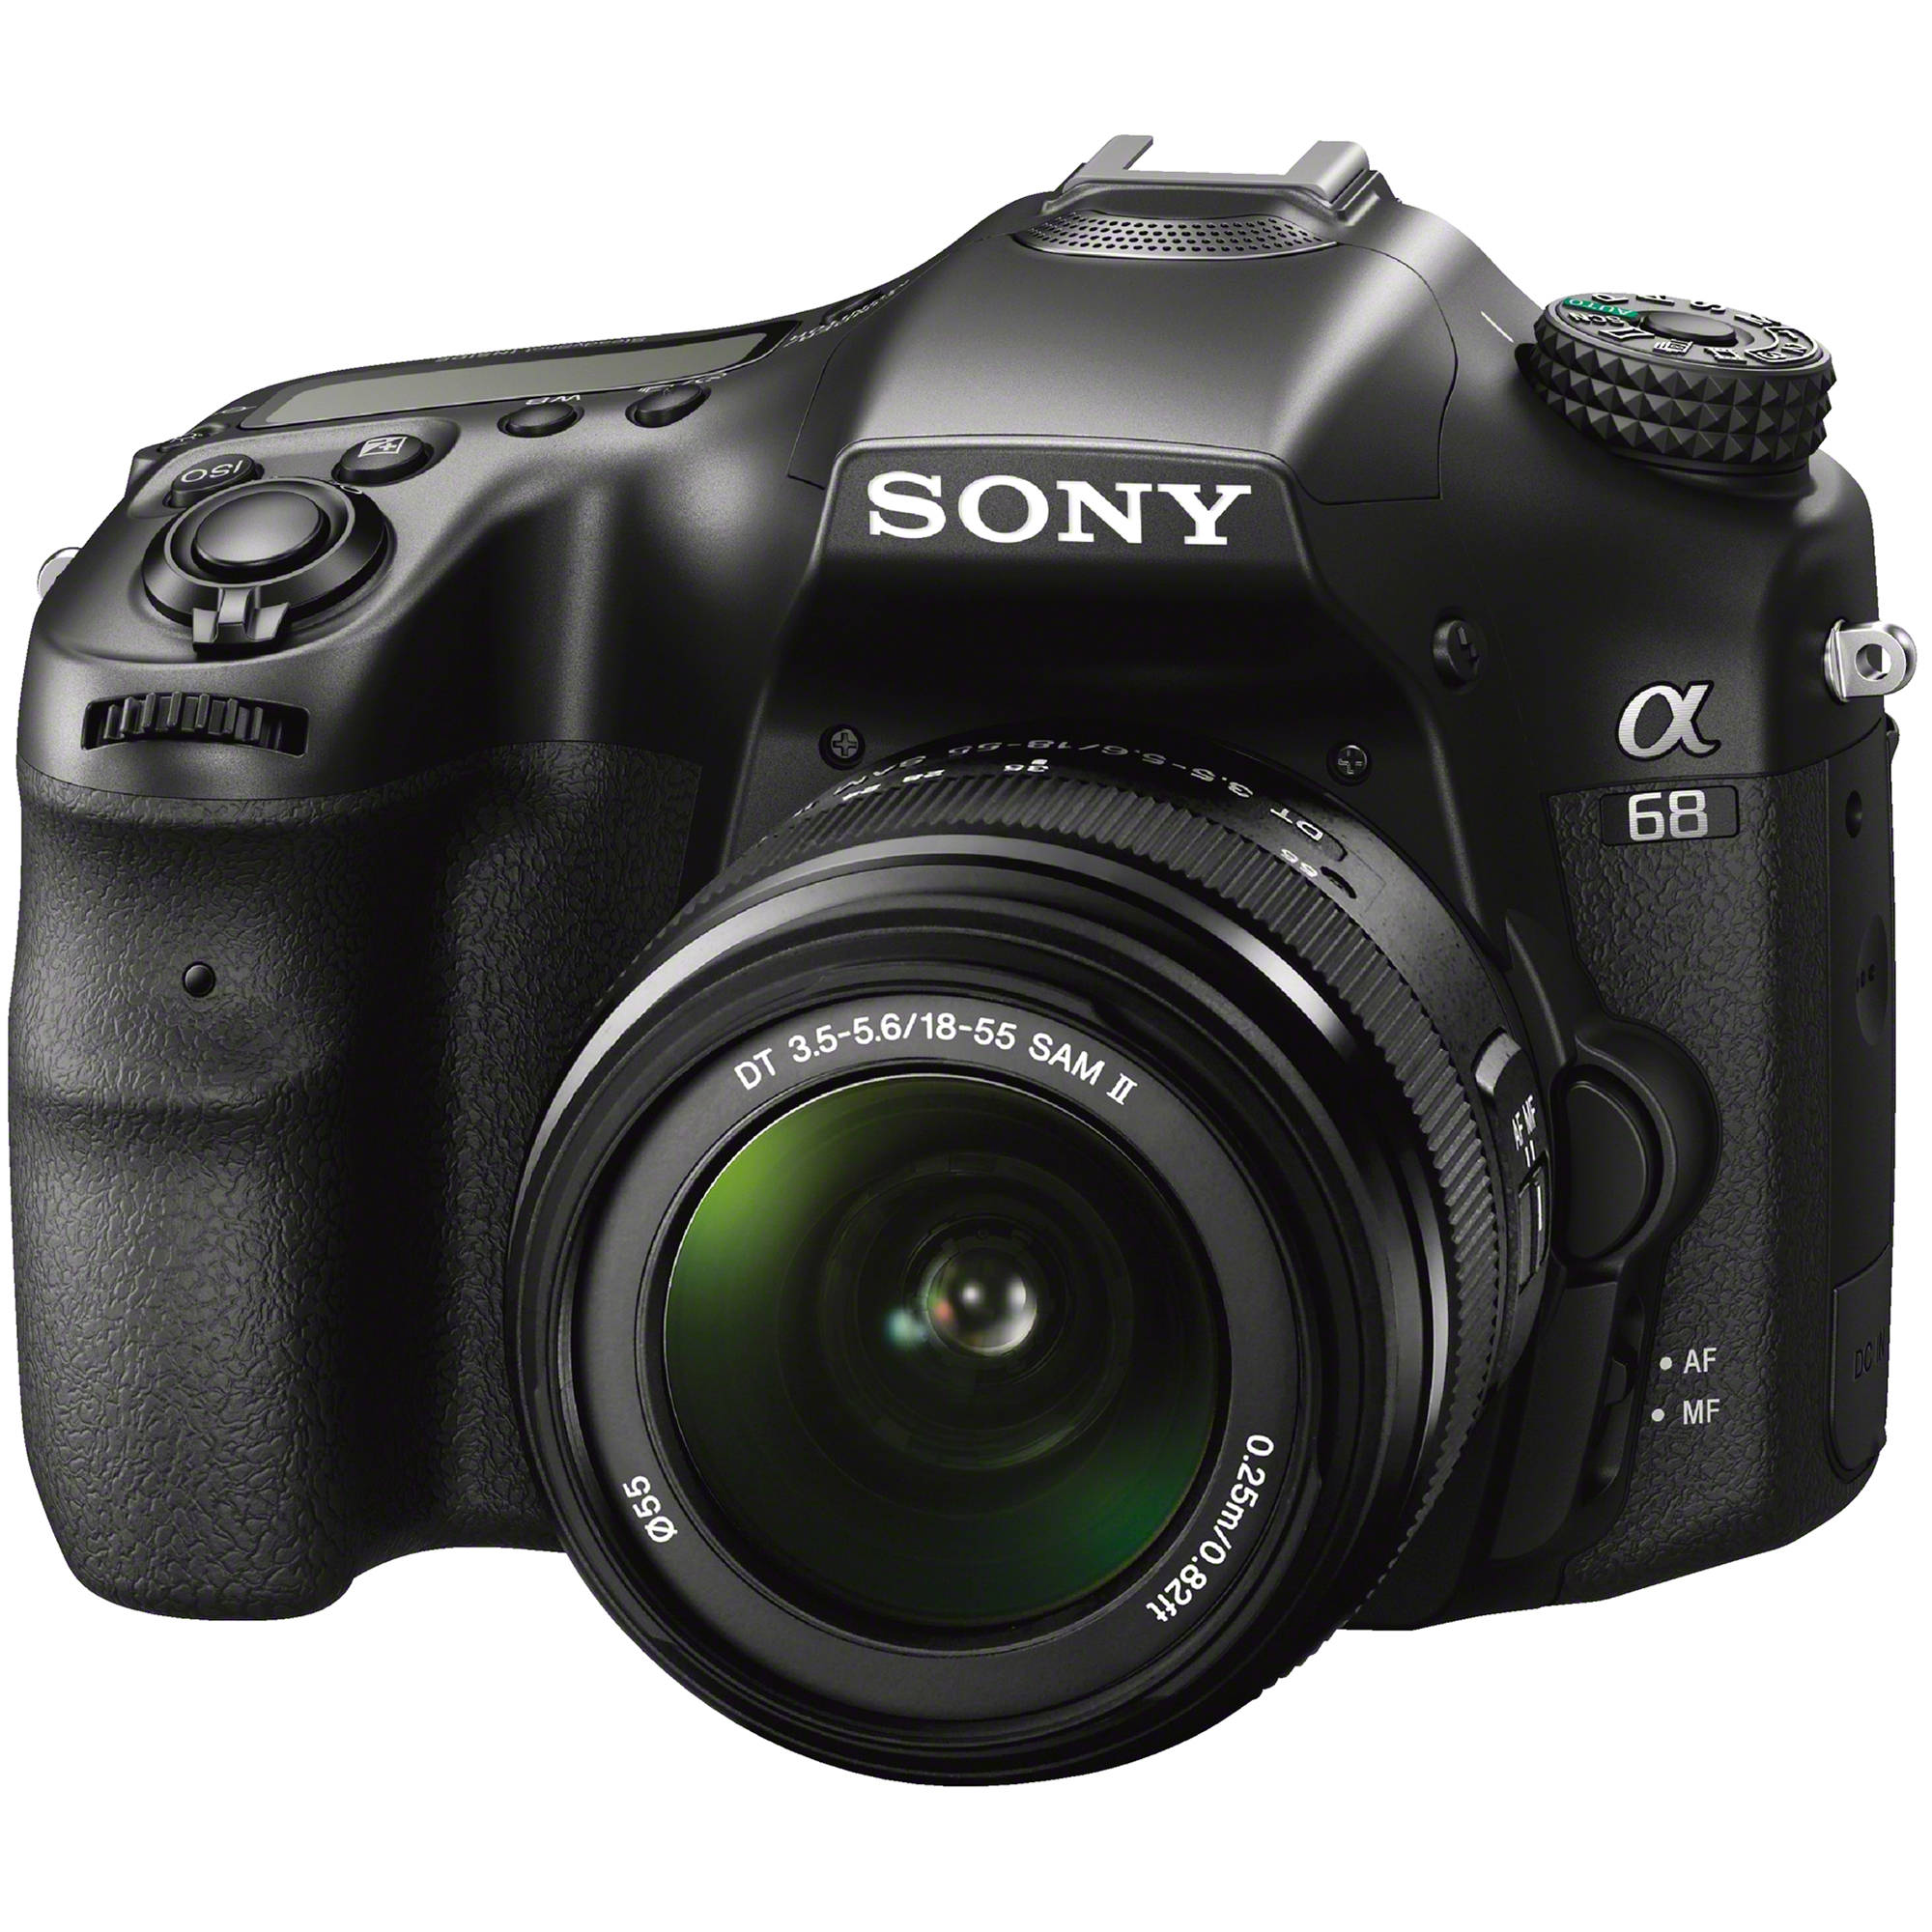
\includegraphics[width=1.0\textwidth]{problem/dslr}
      \end{figure}
    \end{column}
  \end{columns}
\end{frame}


\begin{frame}{Calibration with Checkerboard Patterns}
  \begin{figure}
    \centering
    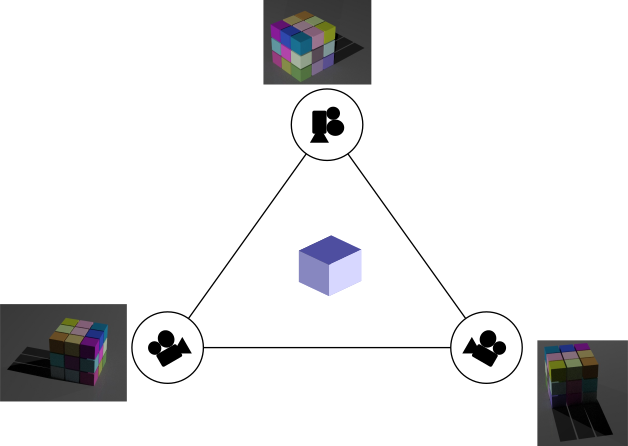
\includegraphics[width=0.7\textwidth]{problem/camera_graph}
  \end{figure}
\end{frame}


\begin{frame}{IMU}
  \begin{figure}
    \centering
    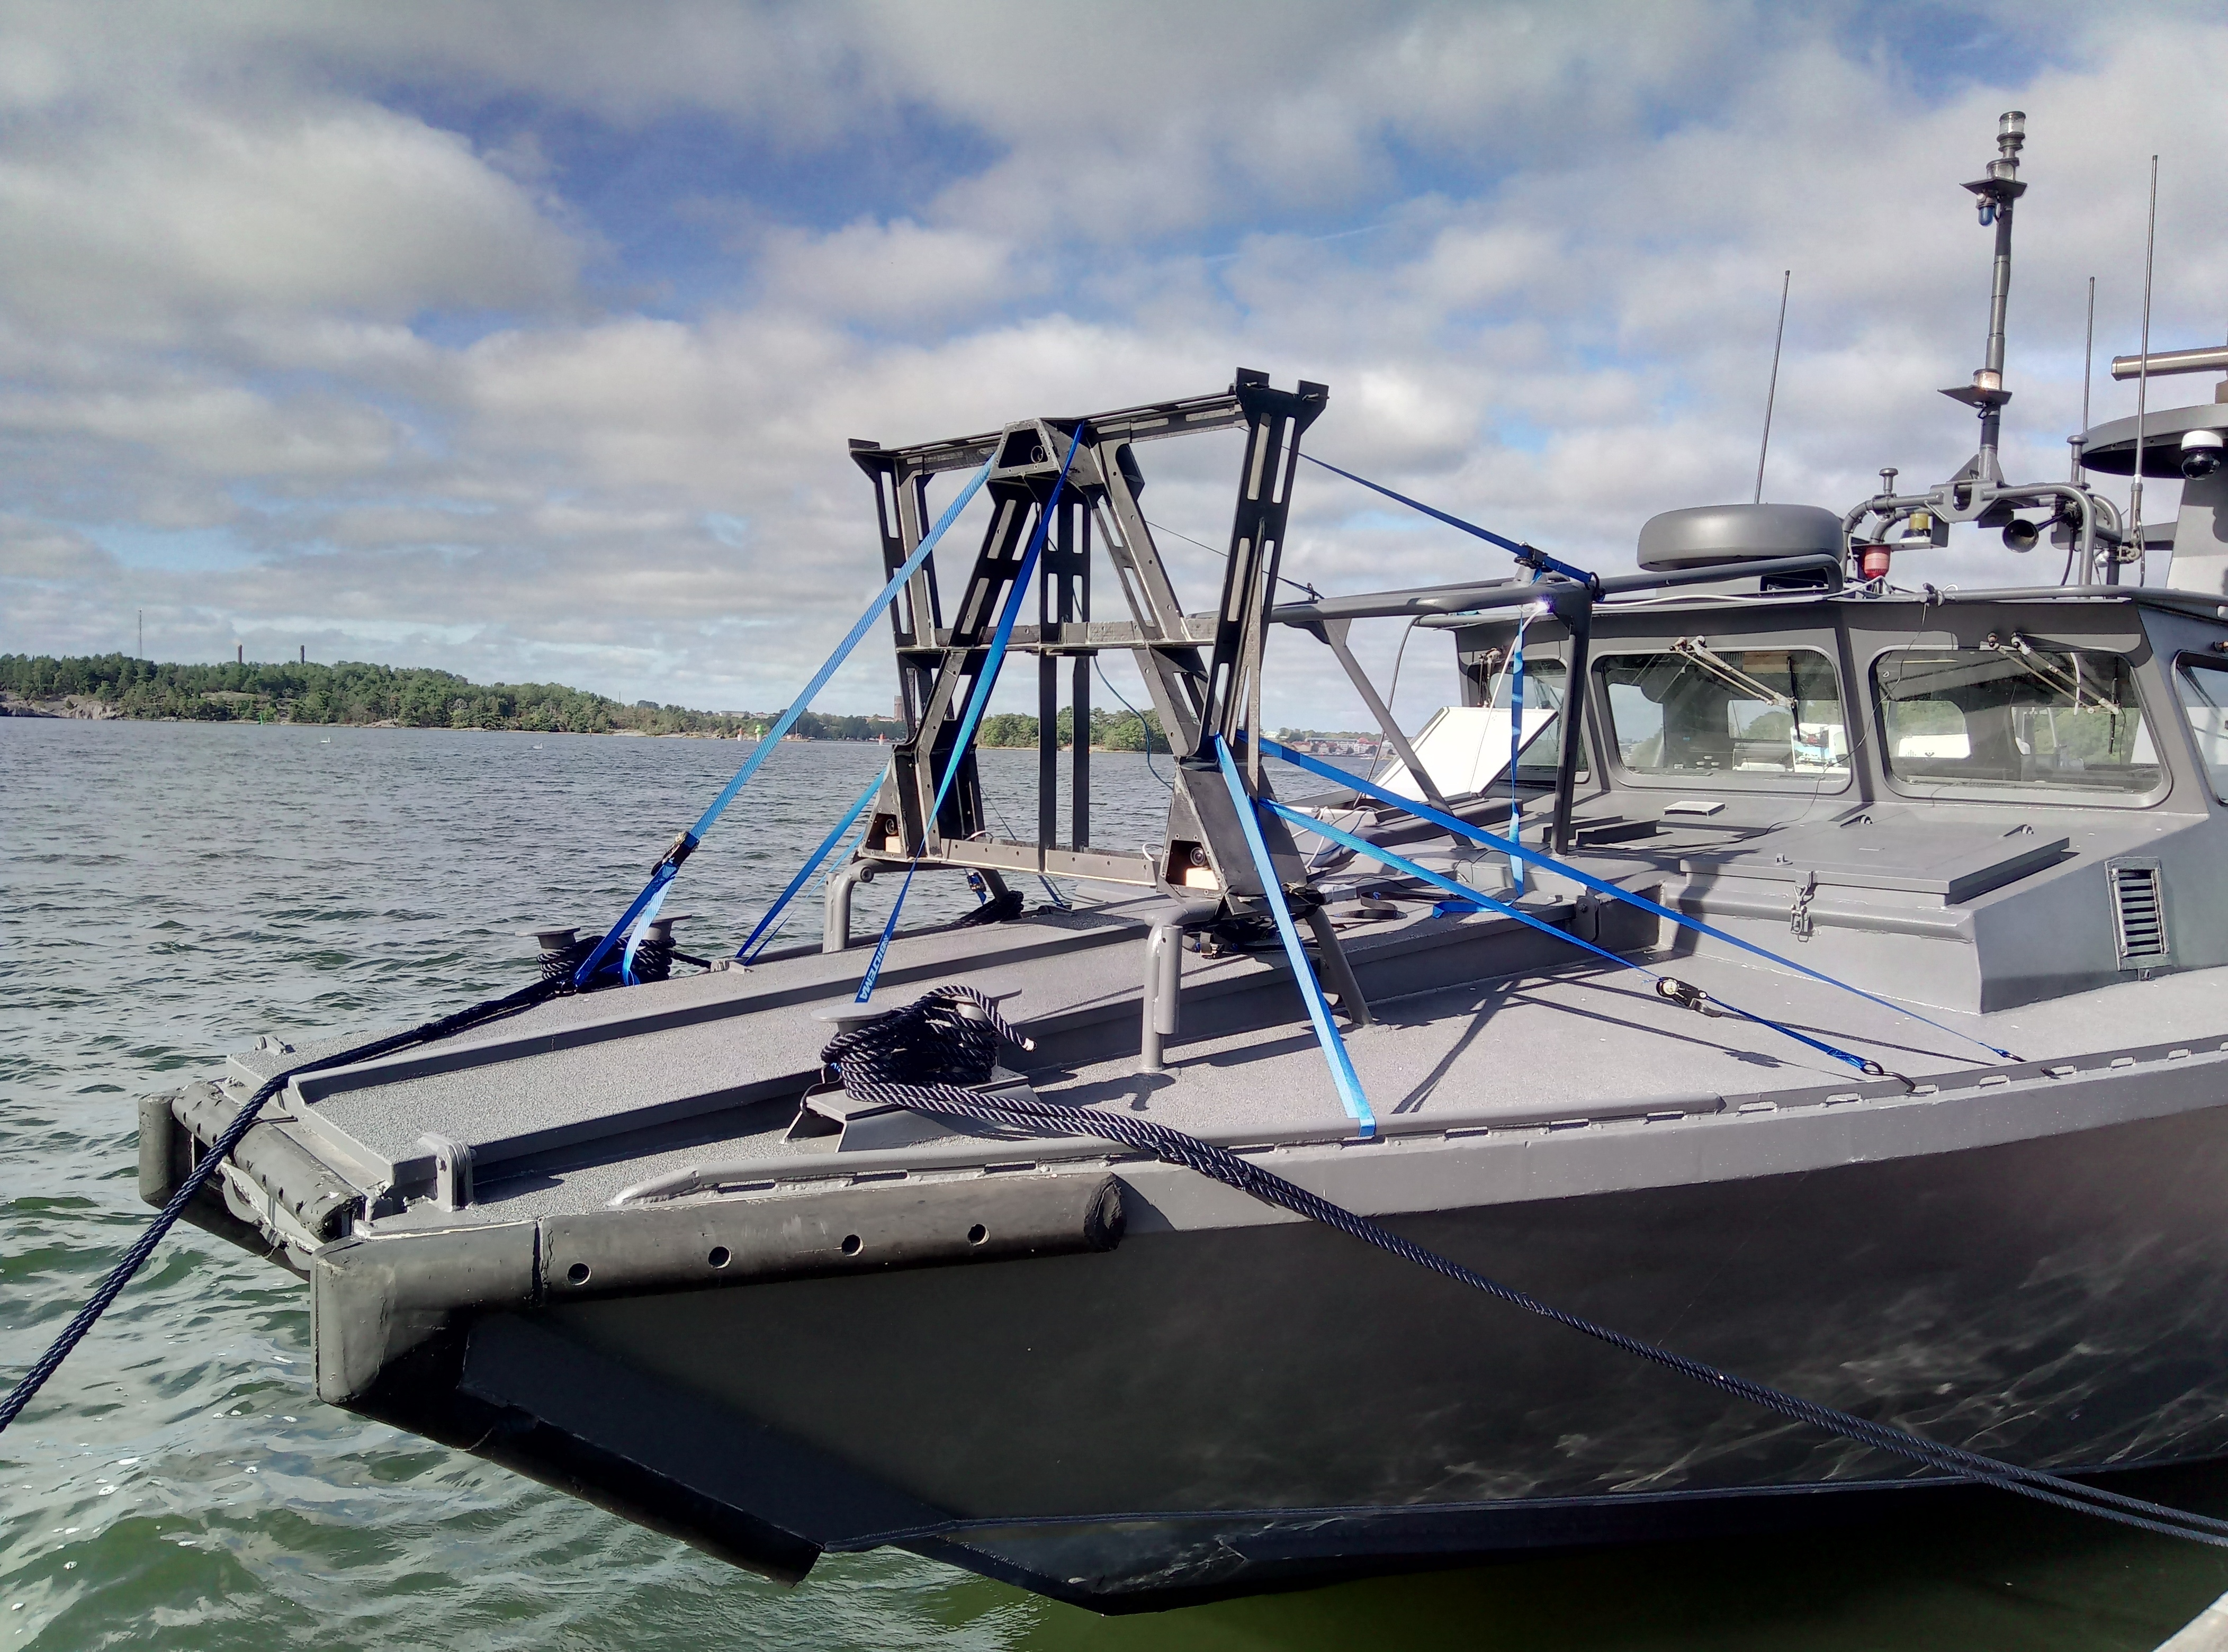
\includegraphics[width=0.7\textwidth]{problem/imu_rig}
  \end{figure}
\end{frame}


\bgroup
\setbeamertemplate{background}{}
\setbeamercolor{background canvas}{bg=black}
% \setbeamertemplate{navigation symbols}{}
\begin{frame}[t,plain]{}{}
  \begin{center}
    {\tiny \textcolor{white}{The End}}
  \end{center}
\end{frame}
\egroup

\end{document}
